% !TEX TS-program = pdflatex
% !TEX encoding = UTF-8 Unicode

\documentclass[12pt]{article}

\usepackage[utf8]{inputenc} 

\usepackage{geometry}
\geometry{a4paper} 
\geometry{margin=0.25in} 
\geometry{portrait}

\usepackage{amsmath}
\usepackage{physics}
\usepackage{tikz} 

\title{tikz-mechanics}
\author{vijayabhaskar badireddi}

\begin{document}

\section*{First section}

\subsection*{figure 1}

\begin{center}
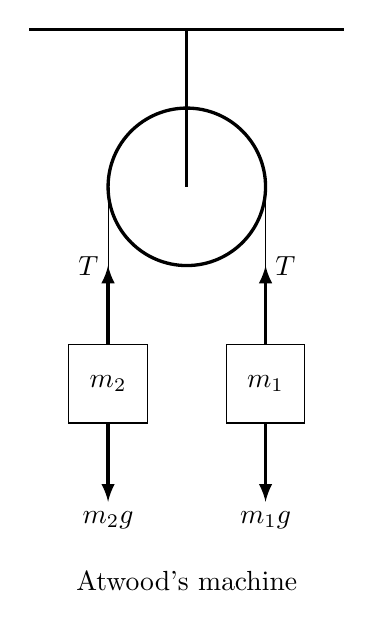
\begin{tikzpicture}[scale=1]
	\draw [very thick] (-2,0) -- (2,0) ;
	\draw [very thick] (0,0) -- (0,-2) ;
	\draw [very thick] (0,-2) circle [radius=1] ;
	\draw (-1,-2) -- (-1,-4) ;
	\draw (1,-2) -- (1,-4) ;
	\draw (-1.5,-4) rectangle (-0.5,-5) ;
	\draw (0.5,-4) rectangle (1.5,-5) ;
	\draw [very thick,-{latex}] (1,-4) -- (1,-3) ;
	\draw [very thick,-{latex}] (-1,-4) -- (-1,-3) ;
	\draw (1,-3) node [anchor=west] {$T$} ;
	\draw (-1,-3) node [anchor=east] {$T$} ;
	\draw (1,-4.5) node {$m_1$} ;
	\draw (-1,-4.5) node {$m_2$} ;
	\draw [very thick,-{latex}] (1,-5) -- (1,-6) ;
	\draw [very thick,-{latex}] (-1,-5) -- (-1,-6) ;
	\draw (1,-6) node [anchor=north] {$m_1g$} ;
	\draw (-1,-6) node [anchor=north] {$m_2g$} ;
	\draw (0,-7) node {Atwood's machine} ;
\end{tikzpicture}
\end{center}

\end{document}
